\documentclass[letter,11pt]{article}

\usepackage[margin=1in]{geometry}
\usepackage[utf8]{inputenc}
\usepackage{color}
\usepackage{xcolor}
\usepackage{amsmath}
\usepackage{amssymb}
\usepackage{amsthm}
\usepackage{hyperref}
\usepackage{graphicx}
\usepackage{tikz}
\usepackage{caption}
\usepackage{float}
\usepackage[shortlabels]{enumitem}
\usetikzlibrary{positioning,arrows.meta}

\usepackage[plain]{algorithm}
\usepackage{algorithmicx}
\usepackage[]{algpseudocode}




\begin{document}

\noindent\rule[2mm]{\textwidth}{1.5mm}
\noindent
\begin{minipage}{.3\textwidth}
  \vspace{-3mm}
  {\Huge\bf HW 6}
\end{minipage}\hfill\begin{minipage}{.5\textwidth}
\begin{flushright}
  {\bf Intro Algorithms EN.601.433 \\
  Fall 2023 \\
  Due: Friday 12/08/2023 at 11:59 PM}%
\vspace{3mm}
\end{flushright}
\end{minipage}
\noindent\rule{\textwidth}{1.5mm}

\section*{Instructions}

\begin{itemize}
\item This homework is worth 10\% of your final grade.

\item This homework is due Friday 12/08/2023 at 11:59 PM on Gradescope.  Solutions will be posted on Canvas at midnight.  No late homework will be accepted.  To access Gradescope, click the Gradescope link on Canvas.

\item You are \textbf{required} to type your homework.  We will
  provide the \LaTeX{} source code to the homework assignments, which you may
  optionally use as a template.  If you install \LaTeX{} on your computer, you can
  generate a PDF of
  your homework by running the command: \\
  \\
  \texttt{latexmk~-pdf~my-homework.tex} \\
  \\
  Alternately, you can use \url{https://www.overleaf.com/edu/jhu} as a web based
  \LaTeX{} editor.

\item You can collaborate with one other person.
    Collaboration should happen through verbal communication, scratch paper,
    whiteboards, etc.  You are \textbf{not} allowed to copy homework
    solutions from another student.  All students are required to submit their
    own write-up.

\item You are \textbf{not} allowed to use any website to find solutions to these problems.

\item Do not write your name on your homework. Instead, write your Johns Hopkins Student ID.  This will allow us to grade your homework anonymously.

\item For questions that require you to write an algorithm out, you can either use pseudo-code or English description.

\item Make sure that you correctly assign which page a problem is located on when uploading to Gradescope.

\item For problems that require graphs or diagrams, you are allowed to include an image of a drawing instead of typesetting the graph.\footnote{If you are using LaTeX, you can follow the instructions here \url{https://www.overleaf.com/learn/latex/Inserting_Images} to embed an image in LaTeX.}

\end{itemize}


\newpage
%%%%%%%%%%%%%%%%%%%%%%%%%%%%%%%%%%%%%%%%%%%%%%%%%%%%%%%%%%%%%%%%%%%%%%%%%%%%%%%%%%%%%%%%%%%%%%%%%%%%
%  _    ___          __  _____           _     _
% | |  | \ \        / / |  __ \         | |   | |
% | |__| |\ \  /\  / /  | |__) | __ ___ | |__ | | ___ _ __ ___  ___
% |  __  | \ \/  \/ /   |  ___/ '__/ _ \| '_ \| |/ _ \ '_ ` _ \/ __|
% | |  | |  \  /\  /    | |   | | | (_) | |_) | |  __/ | | | | \__ \
% |_|  |_|   \/  \/     |_|   |_|  \___/|_.__/|_|\___|_| |_| |_|___/
%%%%%%%%%%%%%%%%%%%%%%%%%%%%%%%%%%%%%%%%%%%%%%%%%%%%%%%%%%%%%%%%%%%%%%%%%%%%%%%%%%%%%%%%%%%%%%%%%%%%

\section{Let There Be Ergonomic Light! (3 points)}
Suppose you’re a consultant for the Ergonomic Architecture Commission,
and they come to you with the following problem. They’re really concerned about designing houses that are “user-friendly,” and they’ve been having a lot of trouble with the setup of light fixtures and switches in newly designed houses.


Consider, for example, a one-floor house with $n$ light fixtures and $n$ locations for light switches mounted in the wall. You’d like to be able to wire up one switch to control each light fixture, in such a way that a person at the switch can see the light fixture being controlled. 
Sometimes this is possible and sometimes it isn’t. Consider the two simple floor plans for houses in Figure \ref{fig:q1}. There are three light fixtures (labeled $a$, $b$, $c$) and three switches (labeled 1, 2, 3). It is possible to wire switches to fixtures in Figure \ref{fig:q1}(a) so that every switch has a line of sight to the fixture, but this is not possible in Figure \ref{fig:q1}{}(b).
\begin{figure}[H]
  \centering
  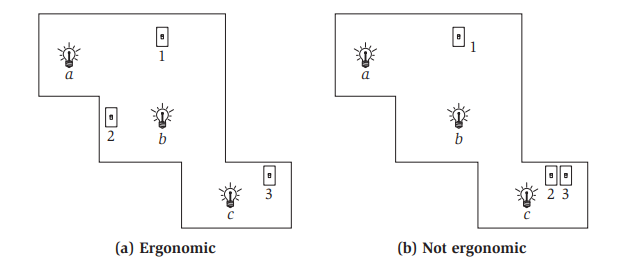
\includegraphics[scale=1]{hw6-q1.png}
    \caption{The floor plan in (a) is ergonomic, because we can wire switches to fixtures in such a way that each fixture is visible from the switch that controls it. (This can be done by wiring switch 1 to $a$, switch 2 to $b$, and switch 3 to $c$.) The floor plan in (b) is not ergonomic, because no such wiring is possible.}
    \label{fig:q1}
\end{figure}
Let’s call a floor plan, together with $n$ light fixture locations and $n$ switch locations, ergonomic if it’s possible to wire one switch to each fixture so that every fixture is visible from the switch that controls it. A floor plan will be represented by a set of $m$ horizontal or vertical
line segments in the plane (the walls), where the $i^{th}$ wall has endpoints ($x_i$, $y_i$), ($x'_i$, $y'_i$). Each of the $n$ switches and each of the $n$ fixtures is given by its coordinates in the plane. A fixture is visible from a switch if the line segment joining them does not cross any of the walls.


Give an algorithm to decide if a given floor plan is ergonomic. The running time should be polynomial in m and n. Provide the total runtime. You may assume that you have a subroutine with $O(1)$ running time that takes two line segments as input and decides whether or not they cross in the plane.

\subsection{Solution}

Let's build a bipartite graph $G = (V,E)$. Split the set of nodes $V$ into sets $X$ and $Y$, representing switches and fixtures respectively. There is an edge from a node in $X$ to a node in $Y$ if and only if the line segment between the switch and fixture that the nodes represent does not intersect any of the $m$ walls in the floor plan. So, creating graph $G$ will take $\mathcal{O}(n^2m)$ time.

Now we can test in $\mathcal{O}(n^3)$ time whether G is a perfect matching, and if so, the fllor plan is ergonomic, because a perfect matching in G is a pairing of switches and fixtures where each switch can see the fixture it is paired with.


\section{Mobile Computing (3 points)}

Consider a set of mobile computing clients in a certain town who each need to be connected to one of several possible base stations. We’ll suppose there are $n$ clients, with the position of each client specified by its $(x, y)$ coordinates in the plane. There are also $k$ base stations; the position of each of these is specified by $(x, y)$ coordinates as well. For each client, we wish to connect it to exactly one of the base stations. Our choice of connections is constrained in the following ways.


There is a range parameter $r$—a client can only be connected to a base station that is within distance $r$. There is also a load parameter $L$—no more than $L$ clients can be connected to any single base station.


Your goal is to design a polynomial-time algorithm for the following problem. Given the positions of a set of clients and a set of base stations, as well as the range and load parameters, decide whether every client can be connected simultaneously to a base station, subject to the range and
load conditions.

\subsection{Solution}

Construct a flow network graph as follows: There is a node for every client, as well as a node for every base station. Add a source node $s$ and a sink node $t$. For every client node, there is an edge from source node to the client node with capacity $1$. For every base station node, there is an edge from the base station node to the sink node with capacity $L$. For every pair of client node and base station node, there is an edge from the client node to the base station node with capacity $1$ if and only if the distance between the client and the base station is at most $R$. Now, we run the Ford-Fulkerson algorithm on this flow network, taking polynomial time. If the value of the max 
flow is same to the number of clients, then every client can be connected.

\section{$k$-Nearest Hospitals (3 points)}

Due to large-scale flooding in a region, paramedics have identified a set of $n$ injured people distributed across the region who need to be rushed to hospitals. There are $k$ hospitals in the region, and each of the $n$ people needs to be brought to a hospital that is within a half-hour’s driving time of their current location (so different people will have different options for hospitals, depending on where they are right now).


At the same time, one doesn’t want to overload any one of the hospitals by sending too many patients its way. The paramedics are in touch by cell phone, and they want to collectively work out whether they can choose a hospital for each of the injured people in such a way that the load on the hospitals is balanced: Each hospital receives at most $\lceil n/k \rceil$ people.

 Give a polynomial-time algorithm that takes the given information about the people’s locations and determines whether this is possible.

\subsection{Solution: Algorithm}

We can solve this using a network flow algorithm. We create a graph as follows: Assume that for every patient $p$, we have nodes that signify said patients, and for every hospital $h$, we have nodes that signify said hospitals. An edge exists between a patient node and a hospital node if and only if the hospital is reachable by the patient in less than half an hour. We set these edges to have flow capacity $1$. Since this is a network flow graph, we also need source and sink nodes. Create a source node $s$ that links to all patient nodes with capacity $1$, and create a sink node $t$ that links to all the hospital nodes with capacity $\frac{n}{k}$ so that the load on the hospitals is balanced.

Now, we run the Ford-Fulkerson Algorithm on the created network flow graph from $s$ to $t$. This can be done in polynomial time because the capacities are integral, and therefore there is an integral flow. If the Ford-Fulkerson algorithm returns a maximum flow of $n$, that means that it is possible to distribute all injured people to hospitals. If Ford-Fulkerson returns a maximum flow that is not $n$, then it is not possible.


\section{Delete $k$ Edges (3 points)}

Consider the following problem. You are given a flow network with unit capacity edges: It consists of a directed graph $G = (V, E)$, a source $s \in V$, and a sink $t \in V$; and $c_e = 1$ for every $e \in E$. You are also given a parameter $k$. 


The goal is to delete $k$ edges so as to reduce the maximum $s-t$ flow in $G$ by as much as possible. In other words, you should find a set of edges $F \subseteq E$ so that $|F| = k$ and the maximum $s-t$ flow in $G' = (V, E - F)$ is as small as possible subject to this. 


Give a polynomial-time algorithm to solve this problem.

\subsection{Solution}

Since the capacity of every edge is $1$, by removing any $k$ edges in a graph, we reduce the capacity of any cut by at most $k$, and so, the min-cut will reduce by at most $k$. Therefore, the max-flow will reduce by at most $k$. As per the min-cut theorem, there are $s-t$ number of cuts with g number of edges. If $g$ is smaller or equal to number of edges to be cut, then simply remove all the edges from the cut $s-t$. By disconnecting $s$ and $t$, the maximum flow reduces to 0. If the value of $g$ is less than $k$, then by removing $k$ number of edges from the min-cut, a cut of $g-k$ will be created. Therefore, the min-cut becomes $g-k$, and so, the max-flow become $g-k$. The computations for computing the min-cut $s-t$ takes polynomial time as per Ford-Fulkerson, and linear time for removing $k$ number of edges. Therefore, the run time of the algorithm is polynomial time.




\section{In Case of Emergency (3 points)}

You are given a directed graph $G = (V, E)$ (picture a network of roads). A certain collection of nodes $X \subset V$ are designated as populated nodes, and a certain other collection $S \subset V$ are designated as safe nodes. (Assume that $X$ and $S$ are disjoint.) In case of an emergency, we want evacuation routes from the populated nodes to the safe nodes. A set of evacuation routes is defined as a set of paths in $G$ so that (i) each node in $X$ is the tail of one path, (ii) the last node on each path lies in $S$, and (iii) the paths do not share any edges. Such a set of paths gives a way for the occupants of the populated nodes to “escape” to $S$, without overly congesting any edge in $G$.


Given $G$, $X$, and $S$, show how to decide in polynomial time whether such a set of evacuation routes exists.

\subsection{Solution}

In a graph $G$, we want to make sure that there is no congestion in the paths. So, set the capacity of every edge in $G$ to $1$. Create a source node $s$, and add $|X|$ unit capacity edges from $s$ to each node in $X$. Creating a sink node $t$, we also add $|X|$ edges from $S$ to $t$, these edges having capacity $|X|$. We then run the Ford-Fulkerson algorithm to find the maximum flow, taking polynomial time. In this case, a set of evacuation routes exists if the maximum flow $= |X|$.

\section{We Are Cooking! (5 points)}

Suppose you and your friend Kayleigh live, together with $n - 2$ other people, at a popular off-campus cooperative apartment, the Academy on Charles. Over the next $n$ nights, each of you is supposed to cook dinner for the co-op exactly once, so that someone cooks on each of the nights.


Of course, everyone has scheduling conflicts with some of the nights (e.g., exams, concerts, etc.), so deciding who should cook on which night becomes a tricky task. For concreteness, let’s label the people $$\{p_1,..., p_n\},$$ the nights $$\{d_1,..., d_n\};$$ and for person $p_i$, there’s a set of nights $S_i \subset \{ d_1,..., d_n \}$ when they are {\it not} able to cook.


A feasible dinner schedule is an assignment of each person in the co-op to a different night, so that each person cooks on exactly one night, there is someone cooking on each night, and if $p_i$ cooks on night $d_j$, then $d_j \notin S_i$. 

\begin{enumerate}

\item [(a)] Describe a bipartite graph G so that G has a perfect matching if and only if there is a feasible dinner schedule for the co-op.


\item[(b)] Your friend Kayleigh takes on the task of trying to construct a feasible dinner schedule. After great effort, she constructs what she claims is a feasible schedule and then heads off to class for the day.


Unfortunately, when you look at the schedule she created, you notice a big problem. $n - 2$ of the people at the co-op are assigned to different nights on which they are available: no problem there. But for the other two people, $p_i$ and $p_j$, and the other two days, $d_k$ and $d_l$, you discover that she has accidentally assigned both $p_i$ and $p_j$ to cook on night $d_k$, and assigned no one to cook on night $d_l$.


You want to fix Kayleigh’s mistake but without having to recompute everything from scratch. Show that it’s possible, using her “almost correct” schedule, to decide in only $O(n^2)$ time whether there exists a feasible dinner schedule for the co-op. (If one exists, you should also output it.)
\end{enumerate}

\subsection{Solution: Part A}

Create a bipartite graph $G=(V,E)$. There is a node representing each person, and a node representing each night. The edges consist of all pairs $(p_i, d_j)$ such that $d_j \notin S_i$. In a perfect matching, every person is paired to one night, no two people are paired with the same night, and each person is available on the night they are paired with. If $G$ has a perfect matching, then it is a feasible dinner schedule. If $G$ is a feasible dinner schedule, consisting of a set of pairs $S = {(p_i, d_j)}$, then each $(p_i, d_j ) \in S$ is an edge of $G$, no two of these pairs share an endpoint in $G$, and hence these edges define a perfect matching in $G$.

\subsection{Solution: Part B}

First, we construct the bipartite graph $G$ from the previous solution. Now, let $Q$ be the set of edges constructed by Kayleigh. We delete the edge $(p_j, d_k)$, so that $Q$ now has size $n - 1$. Since no person or night appears more than once in $Q$ now, this is a matching. Now, we try to find an augmenting path in $G$ with respect to $Q$. If we find one, then increasing $Q$ using the path found gives us a perfect matching of size $n$ which is a feasible dinner schedule. If we cannot find such a path, then that means there is no perfect matching and no feasible dinner schedule. The process of finding an augmenting path takes $\mathcal{O}(|E|) = \mathcal{O}(n^2)$ time.


\end{document}
